\chapter[Resultados Alcançados]{\textbf{R}esultados \textbf{A}lcançados}
%\addcontentsline{toc}{chapter}{Resultados Alcançados}

\textit{Será apresentado neste capítulo a execução dos experimentos sob a solução abordada nas seções anteriores, e exposto os resultados que foram alcançados.}

\section{Materiais e Métodos}

Os experimentos sobre a solução de integração dos sistemas, foram necessários grandes esforços tanto no planejamento de um ambiente controlado quanto na elaboração e análise dos cenários de testes envolvidos. Para que os cenários de teste sejam o mais semelhante ao ambiente de produção os mesmo serão executados sobre uma chamada telefônica tendo como originador o suposto cliente com as devidas características. 

\subsection{Ambiente de teste}

O ambiente para execução dos testes será realizando um terminal cujo as especificações estão descritas abaixo:

\begin{table}[htb]
	\footnotesize
	\caption{Recursos computacionais utilizados}
	\label{tabela:recursosUtilizados}
	\begin{tabular}{|p{3.5cm}|p{3cm}|p{2cm}|p{4cm}|} \hline
		\textbf{SISTEMA OPER.} 	& \textbf{PROCESSADOR} 				& \textbf{MEMÓRIA} 	& \textbf{ARMAZENAMENTO}  \\ \hline
		Windows 7 64 bits 		& Intel Core i7-3520M CPU@2.9GHz 	& 8GB DDR3			& 1TB 5400 rpm \\ \hline
	\end{tabular}
	\legend{\fontsize{10}{12}\selectfont {Fonte: Autoria Própria}.}
\end{table}

Este terminal é responsável em executar ambos os sistemas envolvidos, no entanto como software Asterisk está disponível somente para plataforma Linux será utilizado o recurso de máquina virtual através do software Virtual Box\footnote{Disponível em \url{https://www.virtualbox.org/}}, para subir uma instância da distribuição Disc-Os conforme citado nas seções anteriores.
 
O terminal possui uma conexão de rede local ativa, para que seja atribuído uma faixa de IP ao sistema operacional hospedeiro e ao convidado.
Visando garantir o correto funcionamento e a padronização do ambiente de teste foram criados testes de integração reproduzindo uma chamada telefônica programaticamente simulando um ambiente real, para tanto foi necessário utilizar os seguintes recursos o framework JUnit na construção dos testes e o recurso nativo do Asterisk chamado \textit{Local Channel} que permite criar um canal de comunicação com um contexto e extensão específica dentro do sistema Asterisk, ou seja permite acessar diretamente o ponto de integração entre os sistemas.

Foram criados contextos específicos para teste no software Asterisk, conforme visto abaixo;

\begin{figure}[H]
	\centering
	\caption{Declaração dos contextos de teste no Asterisk}
	\label{figura:contextoTeste}
	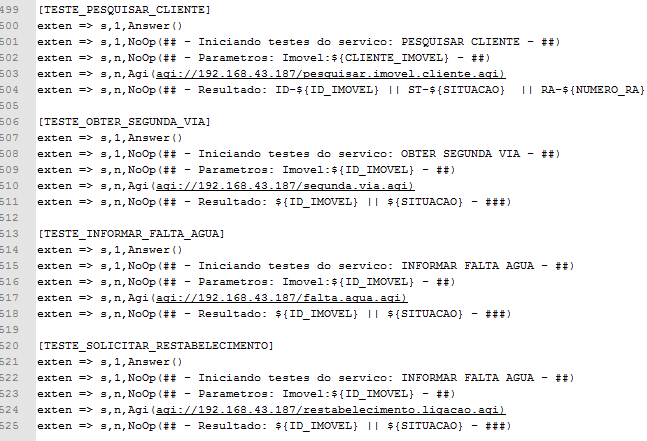
\includegraphics{figuras/contexto_teste.png}
	\legend {\fontsize{10}{12}\selectfont {Fonte: Autoria Própria}.}	
\end{figure}



\subsection{Elaboração dos Cenários de Teste}

Os cenários de testes representam as possíveis situações cadastrais fictícias e comportamentais vinculadas a um cliente, essencial para realizar um atendimento via sistema. Foram propostos 3 cenários de teste para cada serviço automatizado, visando assegurar o correto comportamento da solução. Abaixo estão descritos os cenários conforme cada serviços proposto:

\subsubsection{Obter 2ª Via de Conta}
Abaixo serão descritos os casos de testes previstos para o serviço Obter 2ª Via de Conta.
\begin{flushleft}
	\begin{description}
		\item \textbf{CENÁRIO 1}: Cliente devidamente cadastrado no Sistema, atualmente usuário de um imóvel que possui ativo a Ligação de Água e Esgoto, com uma conta em atraso. O Cliente deseja obter a conta em aberto, conforme demostrado na figura \ref{figura:2ViaCenario1}.
		\begin{figure}[H]
			\centering
			\caption{Obter 2ª via - Cenário de Teste 1}
			\label{figura:2ViaCenario1}
			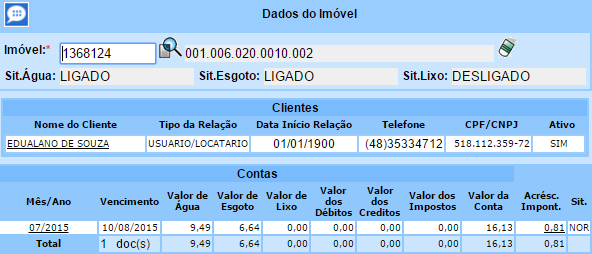
\includegraphics{figuras/cenarios/segunda_via/cenario_1.PNG}
			\legend {\fontsize{10}{12}\selectfont {Fonte: Autoria Própria}.}	
		\end{figure}
	\end{description}
	
	\begin{description}
		\item \textbf{CENÁRIO 2}: Cliente devidamente cadastrado no Sistema, atualmente sendo usuário de um imóvel que possui a Ligação de Água cortada por falta de pagamento, atualmente com três contas em aberto. O Cliente deseja obter todas as contas em aberto, conforme demostrado na figura \ref{figura:2ViaCenario2}.
		\begin{figure}[H]
			\centering
			\caption{Obter 2ª via - Cenário de Teste 2}
			\label{figura:2ViaCenario2}
			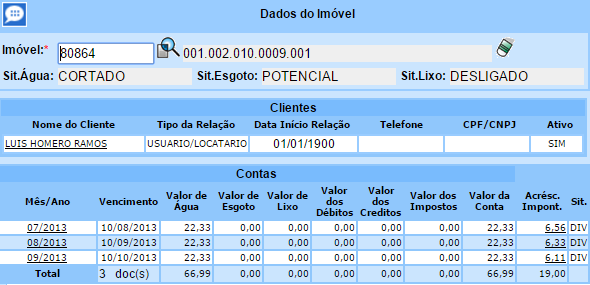
\includegraphics{figuras/cenarios/segunda_via/cenario_2.PNG}
			\legend {\fontsize{10}{12}\selectfont {Fonte: Autoria Própria}.}	
		\end{figure}
	\end{description}
	
	\begin{description}
		\item \textbf{CENÁRIO 3}: Cliente sem e-mail cadastrado no Sistema, atualmente sendo proprietário por dois imóveis que possuem ativo a Ligação de Água, possuindo várias contas pendentes para cada imóvel. O Cliente pretende obter todas as contas de todos os imóveis, conforme demostrado na figura \ref{figura:2ViaCenario3}.
		\begin{figure}[H]
			\centering
			\caption{Obter 2ª via - Cenário de Teste 3}
			\label{figura:2ViaCenario3}
			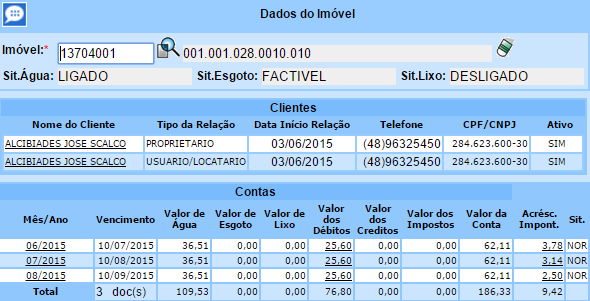
\includegraphics{figuras/cenarios/segunda_via/cenario_3.PNG}
			\legend {\fontsize{10}{12}\selectfont {Fonte: Autoria Própria}.}	
		\end{figure}
	\end{description}
	
\end{flushleft}


\subsubsection{Informar Falta de Água}
Abaixo serão descritos os casos de testes previstos para o serviço Informar Falta de Água.
\begin{flushleft}
	\begin{description}
		\item \textbf{CENÁRIO 1}: Cliente devidamente cadastrado no Sistema, atualmente locatário de um imóvel que possui ativo a Ligação de Água e Esgoto, com pendência de duas contas, com problemas no abastecimento de água. O Cliente pretende informar a falta de água para o imóvel, conforme demostrado na figura \ref{figura:informarFaltaAguaCenario1}.
		\begin{figure}[H]
			\centering
			\caption{Informar Falta de Água - Cenário de Teste 1}
			\label{figura:informarFaltaAguaCenario1}
			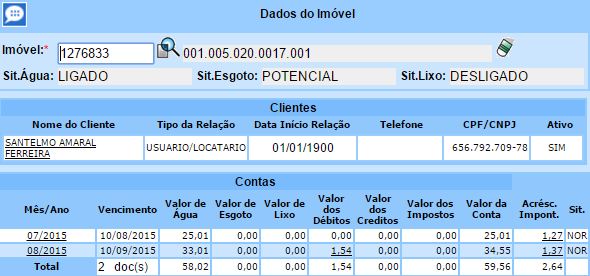
\includegraphics{figuras/cenarios/informar_falta_agua/cenario_1.PNG}
			\legend {\fontsize{10}{12}\selectfont {Fonte: Autoria Própria}.}	
		\end{figure}
	\end{description}
	
	\begin{description}
		\item \textbf{CENÁRIO 2}: Cliente sem e-mail cadastrado no Sistema, atualmente usuário de um único imóvel que possui ativo a Ligação de Água, com situação de adimplência, com problemas no abastecimento de água. O Cliente pretende informar a falta de água para o único imóvel, conforme demostrado na figura \ref{figura:informarFaltaAguaCenario1}.
		\begin{figure}[H]
			\centering
			\caption{Informar Falta de Água - Cenário de Teste 2}
			\label{figura:informarFaltaAguaCenario2}
			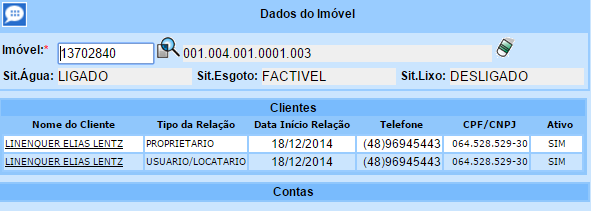
\includegraphics{figuras/cenarios/informar_falta_agua/cenario_2.PNG}
			\legend {\fontsize{10}{12}\selectfont {Fonte: Autoria Própria}.}	
		\end{figure}
		
	\end{description}
	
	\begin{description}
		\item \textbf{CENÁRIO 3}: Cliente devidamente cadastrado no Sistema, atualmente proprietário de dois imóveis, que possuem a Ligação de Água ativa, em situação de inadimplência. O Cliente deseja informar problemas no abastecimento de água do imóvel específico onde reside, conforme demostrado na figura \ref{figura:informarFaltaAguaCenario3}.
		\begin{figure}[H]
			\centering
			\caption{Informar Falta de Água - Cenário de Teste 3}
			\label{figura:informarFaltaAguaCenario3}
			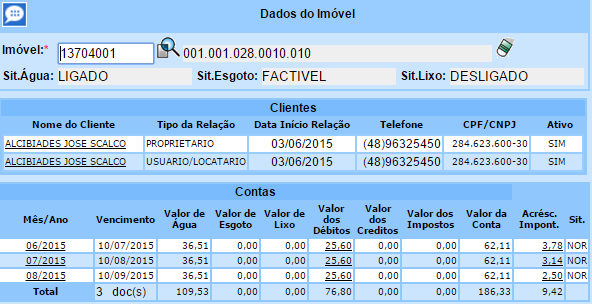
\includegraphics{figuras/cenarios/informar_falta_agua/cenario_3.PNG}
			\legend {\fontsize{10}{12}\selectfont {Fonte: Autoria Própria}.}	
		\end{figure}
	\end{description}
\end{flushleft}	

\subsubsection{Solicitar Restabelecimento da Ligação de Água}
Abaixo serão descritos os casos de testes previstos para o serviço Solicitar Restabelecimento da Ligação de Água.
\begin{flushleft}
	\begin{description}
		\item \textbf{CENÁRIO 1}: Cliente devidamente cadastrado no Sistema, atualmente proprietário de um único imóvel que possui a Ligação de Água interrompida por corte, em situação recente de adimplência. O Cliente deseja solicitar restabelecimento da ligação para o imóvel, conforme demostrado na figura \ref{figura:restabelecimentoLigacaoCenario1}.
		\begin{figure}[H]
			\centering
			\caption{Restabelecimento da Ligação de Água - Cenário de Teste 1}
			\label{figura:restabelecimentoLigacaoCenario1}
			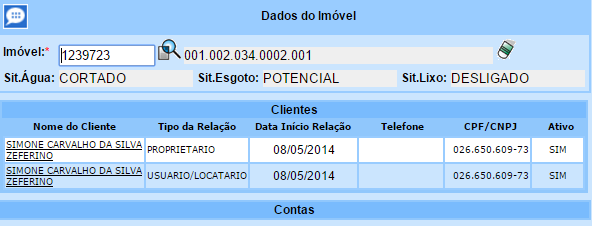
\includegraphics{figuras/cenarios/restabelecimento/cenario_1.PNG}
			\legend {\fontsize{10}{12}\selectfont {Fonte: Autoria Própria}.}	
		\end{figure}
	\end{description}
	
	\begin{description}
		\item \textbf{CENÁRIO 2}: Cliente devidamente cadastrado no Sistema, atualmente usuário de um único imóvel que possui a Ligação de Água interrompida por corte, em situação recente de adimplência. O Cliente deseja solicitar restabelecimento da ligação para o imóvel, conforme demostrado na figura \ref{figura:restabelecimentoLigacaoCenario2}.
		\begin{figure}[H]
			\centering
			\caption{Restabelecimento da Ligação de Água - Cenário de Teste 2}
			\label{figura:restabelecimentoLigacaoCenario2}
			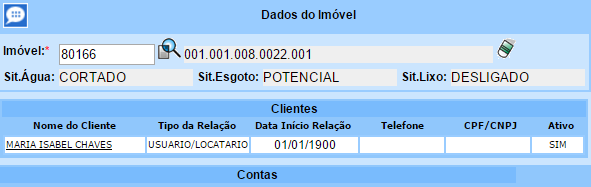
\includegraphics{figuras/cenarios/restabelecimento/cenario_2.PNG}
			\legend {\fontsize{10}{12}\selectfont {Fonte: Autoria Própria}.}	
		\end{figure}
	\end{description}
	
	\begin{description}
		\item \textbf{CENÁRIO 3}: Cliente devidamente cadastrado no Sistema, atualmente proprietário de um imóvel, que possui Ligação de Água interrompida por corte, devido a falta de pagamento das várias contas em aberto. O Cliente deseja solicitar restabelecimento da ligação para o imóvel sem realizar a negociação das faturas, conforme demostrado na figura \ref{figura:restabelecimentoLigacaoCenario3}.
		\begin{figure}[H]
			\centering
			\caption{Restabelecimento da Ligação de Água - Cenário de Teste 3}
			\label{figura:restabelecimentoLigacaoCenario3}
			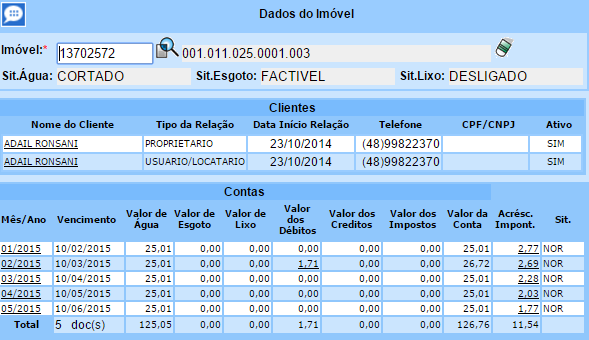
\includegraphics{figuras/cenarios/restabelecimento/cenario_3.PNG}
			\legend {\fontsize{10}{12}\selectfont {Fonte: Autoria Própria}.}	
		\end{figure}
	\end{description}

\end{flushleft}	


\subsection{Execução dos Cenários de Teste}
A execução dos cenários propostos será feita utilizando os testes automatizados citados na seção anterior, cada resultado será coletado e apresentado. 

TODO: ATUALIZAR COM AS IMAGENS!!


\subsection{Análise dos resultados}
O cenário deve ser totalmente atendimento para que se tenha sucesso no atendimento e posteriormente a situação de \textbf{ATENDINDO}, caso contrário será obtido à situação de \textbf{NÃO ATENDINDO}, caso o atendimento não seja concluído com sucesso o cenário deve conter uma observação, descrevendo o motivo ao qual levou a tal situação.
Abaixo serão descritos os Cenários dos serviços propostos:




